\documentclass[aspectratio=169,11pt]{beamer}

\usetheme{SimplePlus}

\usepackage{amsmath}
\usepackage{amssymb}
\usepackage{booktabs}
\usepackage{graphicx}
\usepackage{array}

\graphicspath{{images/lecture-2/}}

\title{S181M116 Derivatives and Alternative Investments}
\subtitle{Lecture 2: Hedging with Futures and Forward/Futures Prices}
\author{Swapnil Singh}
\institute{Lietuvos Bankas and Kaunas University of Technology}
\date{}

\newcommand{\St}{S_T}
\newcommand{\Szero}{S_0}
\newcommand{\Ft}{F_t}
\newcommand{\Fzero}{F_0}
\newcommand{\K}{K}
\newcommand{\Var}{\operatorname{Var}}
\newcommand{\Cov}{\operatorname{Cov}}
\newcommand{\E}{\mathbb{E}}

\AtBeginSection[]{
    \begin{frame}[plain,noframenumbering]
        \vfill
        \begin{center}
            {\usebeamerfont{subtitle}\usebeamercolor[fg]{structure}Section \thesection\par}
            \vspace{0.5em}
            {\usebeamerfont{title}\usebeamercolor[fg]{titlelike}\insertsectionhead\par}
        \end{center}

        \vspace{1.2em}
        \begin{center}
            \begin{minipage}{0.72\textwidth}
                \tableofcontents[currentsection,hideothersubsections]
            \end{minipage}
        \end{center}
        \vfill
    \end{frame}
}

\begin{document}

\begin{frame}
    \titlepage
\end{frame}

\begin{frame}{Today}
    \begin{enumerate}
        \item How to choose a short hedge or a long hedge.
        \item Why hedges remain imperfect because of basis risk.
        \item How to size cross hedges.
        \item How no-arbitrage determines forward and futures prices.
        \item Why commodity pricing needs storage costs and convenience yield.
        \item How stock-index futures can hedge or change portfolio beta.
        \item Why stack-and-roll hedging creates roll and funding risk.
    \end{enumerate}
\end{frame}

\begin{frame}{Core Message}
    \begin{block}{Lecture 2 has two linked problems}
        \begin{enumerate}
            \item \textbf{Hedging:} choose a futures position that offsets an exposure.
            \item \textbf{Pricing:} explain why spot and futures prices should move together.
        \end{enumerate}
    \end{block}

    \vspace{0.5em}
    A hedge does not make the firm win in every state.
    It trades upside for downside protection, and the remaining gap is usually basis risk.
\end{frame}

\section{Hedge Mechanics}

\begin{frame}{Exposure Comes First}
    Before choosing a futures position, ask:
    \begin{itemize}
        \item Will the firm \textbf{sell} the asset later or \textbf{buy} it later?
        \item Is the futures contract written on the \textbf{same asset}, or only on a \textbf{related asset}?
        \item Do quantity, timing, location, and currency match the exposure?
    \end{itemize}

    \vspace{0.3em}
    If it is only a related asset, the firm is using a \textbf{cross hedge}, so the hedge will be less exact.

    \vspace{0.7em}
    \begin{columns}[T]
        \begin{column}{0.48\textwidth}
            \begin{block}{Short hedge}
                Use a short futures position when the firm owns, produces, or expects to receive an asset that it will later sell.
            \end{block}
        \end{column}
        \begin{column}{0.48\textwidth}
            \begin{block}{Long hedge}
                Use a long futures position when the firm expects to buy an asset later and wants protection against rising prices.
            \end{block}
        \end{column}
    \end{columns}
\end{frame}

\begin{frame}{Short Hedge Example}
    \small
    An oil producer will sell 500,000 barrels in three months.
    The futures price is USD 78 per barrel and each contract is 1,000 barrels, so
    \[
        N=\frac{500{,}000}{1{,}000}=500
    \]
    short contracts are needed.

    \begin{columns}[T]
        \begin{column}{0.48\textwidth}
            \textbf{If spot and futures finish near 72}
            \begin{itemize}
                \item Physical sale: USD 36.0m
                \item Futures gain: USD 3.0m
                \item Total revenue: USD 39.0m
            \end{itemize}
        \end{column}
        \begin{column}{0.48\textwidth}
            \textbf{If spot and futures finish near 84}
            \begin{itemize}
                \item Physical sale: USD 42.0m
                \item Futures loss: USD 3.0m
                \item Total revenue: USD 39.0m
            \end{itemize}
        \end{column}
    \end{columns}

    \begin{block}{Lesson}
        Ignoring basis risk, the short hedge locks in approximately the initial futures price.
    \end{block}
\end{frame}

\begin{frame}{Long Hedge Example}
    \small
    A manufacturer will buy 250,000 pounds of copper in four months.
    The futures price is USD 3.70 per pound and each contract covers 25,000 pounds, so
    \[
        N=\frac{250{,}000}{25{,}000}=10
    \]
    long contracts are needed.

    \begin{columns}[T]
        \begin{column}{0.48\textwidth}
            \textbf{If copper rises to 4.10}
            \begin{itemize}
                \item Physical purchase: USD 1.025m
                \item Futures gain: USD 0.100m
                \item Net cost: USD 0.925m
            \end{itemize}
        \end{column}
        \begin{column}{0.48\textwidth}
            \textbf{If copper falls to 3.40}
            \begin{itemize}
                \item Physical purchase is cheaper.
                \item The futures position loses.
                \item Net cost is still close to USD 3.70 per pound.
            \end{itemize}
        \end{column}
    \end{columns}

    \begin{block}{Rule of Thumb}
        If the firm's exposure moves roughly \textbf{one-for-one} with the asset price,
        a \textbf{fixed number of futures contracts} often works well.
        If the exposure itself changes with price or time, a fixed futures hedge is
        usually not enough, so use \textbf{options} or \textbf{dynamic rebalancing}.
    \end{block}
\end{frame}

\begin{frame}{Why Firms Hedge}
    \begin{columns}[T]
        \begin{column}{0.50\textwidth}
            \begin{block}{Economic reasons}
                \begin{itemize}
                    \item Reduce input-cost or revenue volatility.
                    \item Improve budgeting and investment planning.
                    \item Hedge more cheaply than many individual shareholders can.
                    \item Reduce distress and funding risk from volatile cash flow.
                \end{itemize}
            \end{block}
        \end{column}
        \begin{column}{0.50\textwidth}
            \begin{alertblock}{Common mistake}
                Judge the \textbf{combined} business-plus-futures outcome.
                A hedge can lose money on the futures account precisely because it protected the underlying business exposure.
            \end{alertblock}
        \end{column}
    \end{columns}

    \vspace{0.4em}
    Hedging can even be counterproductive if the firm's margins already adjust naturally with input prices.
\end{frame}

\section{Basis Risk}

\begin{frame}{Basis Risk}
    \begin{columns}[T]
        \begin{column}{0.55\textwidth}
            \begin{block}{Definition}
                \[
                    b_t=S_t-F_t
                \]
                where basis means \textbf{spot minus futures}.
            \end{block}

            \begin{itemize}
                \item Spot and futures prices usually move together.
                \item For the same deliverable asset, basis should be close to zero at true futures maturity.
                \item But firms often close hedges before maturity, or hedge with an imperfect match.
                \item So the basis at \textbf{hedge close} can still be nonzero; that uncertainty is \textbf{basis risk}.
            \end{itemize}
        \end{column}
        \begin{column}{0.41\textwidth}
            \begin{center}
                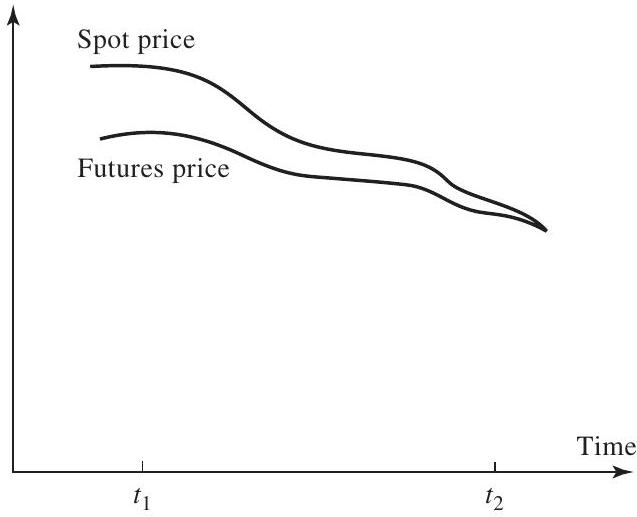
\includegraphics[width=\linewidth,height=0.60\textheight,keepaspectratio]{da7d1f4c-f02d-4245-82cc-df26ce412cbf-076_517_637_1628_455.jpg}
            \end{center}
        \end{column}
    \end{columns}
\end{frame}

\begin{frame}{Effective Sale Price in a Short Hedge}
    \small
    \begin{columns}[T]
        \begin{column}{0.48\textwidth}
            \begin{block}{Cash-flow logic}
                Sell the physical asset later at spot price \(S_2\).
                Short futures gain:
                \[
                    F_1-F_2
                \]
                Effective sale price:
                \[
                    S_2+(F_1-F_2)=F_1+b_2
                \]
                where \(b_2=S_2-F_2\).
            \end{block}

            \begin{exampleblock}{Example}
                \[
                    \underbrace{5.85}_{\text{spot sale}}
                    +
                    \underbrace{(6.20-5.95)}_{\text{futures gain}}
                    =
                    6.10
                \]
            \end{exampleblock}
        \end{column}
        \begin{column}{0.48\textwidth}
            \begin{alertblock}{Intuition}
                \begin{itemize}
                    \item The firm does \textbf{not} pre-sell the physical asset at \(F_1\).
                    \item It still sells later at the market price \(S_2\).
                    \item The short futures position adds cash when prices fall.
                    \item If \(b_2=0\), the effective sale price is exactly \(F_1\); otherwise basis risk is the remaining gap.
                \end{itemize}
            \end{alertblock}
        \end{column}
    \end{columns}
\end{frame}

\begin{frame}{Effective Purchase Price in a Long Hedge}
    \small
    \begin{columns}[T]
        \begin{column}{0.48\textwidth}
            \begin{block}{Cash-flow logic}
                Buy the physical asset later at spot price \(S_2\).
                Long futures gain:
                \[
                    F_2-F_1
                \]
                Effective purchase price:
                \[
                    S_2-(F_2-F_1)=F_1+b_2
                \]
                where \(b_2=S_2-F_2\).
            \end{block}

            \begin{exampleblock}{Example}
                \[
                    \underbrace{3.92}_{\text{spot purchase}}
                    -
                    \underbrace{(3.88-3.70)}_{\text{futures gain}}
                    =
                    3.74
                \]
            \end{exampleblock}
        \end{column}
        \begin{column}{0.48\textwidth}
            \begin{alertblock}{Intuition}
                \begin{itemize}
                    \item The firm does \textbf{not} buy the physical asset today at \(F_1\).
                    \item It still buys later at the market price \(S_2\).
                    \item The long futures position reimburses part of the purchase when prices rise.
                    \item If \(b_2=0\), the effective purchase price is exactly \(F_1\); otherwise basis determines whether it ends above or below \(F_1\).
                \end{itemize}
            \end{alertblock}
        \end{column}
    \end{columns}
\end{frame}

\begin{frame}{Cross Hedging}
    \begin{block}{When is a cross hedge used?}
        When there is no liquid futures contract on the exact exposure, hedge with a related asset instead.
    \end{block}

    \begin{exampleblock}{Example}
        An airline may hedge jet fuel with heating-oil futures if jet-fuel futures are illiquid.
    \end{exampleblock}

    \[
        S_2-F_2=(S_2-S_2^*)+(S_2^*-F_2)
    \]

    \begin{itemize}
        \item The first term is the mismatch between the two physical assets.
        \item The second term is the usual basis for the futures underlying.
        \item Cross hedges therefore add one more source of imperfection.
    \end{itemize}
\end{frame}

\begin{frame}[label=mvhr-main]{Minimum-Variance Hedge Ratio}
    \footnotesize
    If a short hedge uses ratio $h$, the change in the hedged position is
    \[
        \Delta V=\Delta S+h(-\Delta F)=\Delta S-h\Delta F,
    \]
    because a short futures position changes by \(-\Delta F\): it offsets the spot exposure instead of adding to it.

    Choose $h$ to make the residual risk as small as possible:
    \[
        \Var(\Delta V)=\sigma_S^2+h^2\sigma_F^2-2h\Cov(\Delta S,\Delta F).
    \]

    \begin{block}{Optimal hedge ratio}
        \[
            h^*=\frac{\Cov(\Delta S,\Delta F)}{\Var(\Delta F)}
            =\rho\frac{\sigma_S}{\sigma_F}.
        \]
    \end{block}

    \centering
    \hyperlink{mvhr-appendix}{\beamerbutton{Full derivation in appendix}}

    \begin{columns}[T]
        \begin{column}{0.48\textwidth}
            \begin{alertblock}{Intuition}
                \begin{itemize}
                    \item Small $h$: under-hedged.
                    \item Large $h$: futures add noise.
                    \item $h^*$ minimizes residual variance.
                \end{itemize}
            \end{alertblock}
        \end{column}
        \begin{column}{0.48\textwidth}
            \begin{block}{Regression view}
                In \(\Delta S=a+h^*\Delta F+\varepsilon\), the slope is the best-fit hedge ratio.
            \end{block}
        \end{column}
    \end{columns}
\end{frame}

\begin{frame}{From Hedge Ratio to Contracts}
    \footnotesize
    \begin{block}{Contract count}
        \[
            N^*=h^*\frac{Q_A}{Q_F}
            \qquad \text{or} \qquad
            N^*=h^*\frac{V_A}{V_F}.
        \]
    \end{block}

    \begin{exampleblock}{Jet-fuel cross hedge}
        If $\rho=0.80$, $\sigma_S=0.18$, and $\sigma_F=0.15$, then
        \[
            h^*=0.80\frac{0.18}{0.15}=0.96.
        \]
        Hedging 3,000,000 gallons with 42,000-gallon contracts gives
        \[
            N^*=0.96\frac{3{,}000{,}000}{42{,}000}\approx 68.6,
        \]
        so the airline uses about 68 or 69 contracts.
    \end{exampleblock}

    If the regression uses percentage returns, base the contract count on values rather than physical quantities.
\end{frame}

\section{Forward and Futures Pricing}

\begin{frame}{Investment Assets, Consumption Assets, and No-Arbitrage}
    \begin{columns}[T]
        \begin{column}{0.48\textwidth}
            \begin{block}{Investment assets}
                Stocks, bonds, gold, and silver are widely held for investment.
                Cash-and-carry arbitrage often pins down the forward price tightly.
            \end{block}
        \end{column}
        \begin{column}{0.48\textwidth}
            \begin{block}{Consumption assets}
                Oil, copper, gas, wheat, and electricity are held for use.
                Physical ownership can provide convenience benefits that a futures contract does not.
            \end{block}
        \end{column}
    \end{columns}

    \vspace{0.4em}
    For a non-income-paying investment asset,
    \[
        F_0=S_0e^{rT}.
    \]

    Benchmark assumptions: no transaction costs, same borrowing and lending rate, short selling when needed, known income or storage costs, and no default risk.
\end{frame}

\begin{frame}{Cash-and-Carry Arbitrage}
    \small
    Suppose $S_0=80$, $r=4\%$ continuously compounded, and $T=0.75$.
    Then the fair forward price is
    \[
        F_0=80e^{0.04\times 0.75}=80e^{0.03}\approx 82.44.
    \]

    \begin{columns}[T]
        \begin{column}{0.48\textwidth}
            \begin{block}{If the quoted forward is 85}
                \begin{enumerate}
                    \item Borrow 80.
                    \item Buy the stock.
                    \item Short the forward.
                \end{enumerate}
                At maturity, profit is
                \[
                    85-82.44=2.56.
                \]
            \end{block}
        \end{column}
        \begin{column}{0.48\textwidth}
            \begin{block}{If the quoted forward is 81}
                \begin{enumerate}
                    \item Short the stock.
                    \item Invest the proceeds.
                    \item Go long the forward.
                \end{enumerate}
                At maturity, profit is
                \[
                    82.44-81=1.44.
                \]
            \end{block}
        \end{column}
    \end{columns}
\end{frame}

\begin{frame}{Income and Yield in Forward Pricing}
    \small
    \begin{block}{Known cash income}
        \[
            F_0=(S_0-I)e^{rT}
        \]
        Example: $S_0=100$, known dividend PV $I\approx 2.93$, $r=5\%$, $T=1$:
        \[
            F_0=(100-2.93)e^{0.05}\approx 102.05.
        \]
    \end{block}

    \begin{block}{Known yield}
        \[
            F_0=S_0e^{(r-q)T}
        \]
        Useful for stock indices and foreign currencies, where holding the asset gives a running benefit.
    \end{block}
\end{frame}


\begin{frame}{Value of an Existing Forward Contract}
    \small
    \textbf{Old versus new:} An old forward contract has delivery price $K$ fixed in the past. A new forward entered today would have delivery price $F_0$ and zero value today.

    \medskip
    \textbf{At maturity:}
    \[
        \text{old long payoff}=S_T-K,\qquad
        \text{new long payoff}=S_T-F_0.
    \]
    So the old contract is better by
    \[
        (S_T-K)-(S_T-F_0)=F_0-K.
    \]

    \medskip
    This difference is known today but paid at maturity, so its value today is
    \[
        f=(F_0-K)e^{-rT}.
    \]

    \medskip
    \textbf{Example:} if your old long forward lets you buy at $50$ while a new forward today would lock in $54$, then your contract is favorable:
    \[
        f=(54-50)e^{-0.04\times 0.5}\approx 3.92.
    \]
\end{frame}

\begin{frame}{Commodity Pricing: Storage and Convenience Yield}
    \small
    \begin{columns}[T]
        \begin{column}{0.48\textwidth}
            \begin{block}{Storage cost}
                Fixed storage cost PV $U$:
                \[
                    F_0=(S_0+U)e^{rT}
                \]
                Proportional storage cost $u$:
                \[
                    F_0=S_0e^{(r+u)T}
                \]
            \end{block}
        \end{column}
        \begin{column}{0.48\textwidth}
            \begin{block}{Convenience yield}
                Physical inventory can keep production running or protect against shortages.
                With proportional storage cost $u$ and convenience yield $y$:
                \[
                    F_0=S_0e^{(r+u-y)T}.
                \]
            \end{block}
        \end{column}
    \end{columns}

    \begin{exampleblock}{Oil example}
        If $S_0=80$, $r=5\%$, $u=1\%$, $y=4\%$, and $T=0.5$,
        \[
            F_0=80e^{(0.05+0.01-0.04)(0.5)}\approx 80.80.
        \]
        Without convenience yield, the price would be about 82.44.
    \end{exampleblock}
\end{frame}

\begin{frame}{Commodity Curves and Arbitrage Bounds}
    \begin{columns}[T]
        \begin{column}{0.49\textwidth}
            \begin{block}{Investment commodity}
                Gold or silver can often be priced closely by arbitrage from spot, financing, and storage costs.
            \end{block}

            \begin{block}{Consumption commodity}
                For oil or copper, arbitrage may give only an upper bound:
                \[
                    F_0\leq (S_0+U)e^{rT}.
                \]
                A low futures price is not automatically an arbitrage opportunity because inventory has convenience value.
            \end{block}
        \end{column}
        \begin{column}{0.47\textwidth}
            \begin{block}{Curve shape}
                \textbf{Contango:} futures prices rise with maturity.

                \vspace{0.4em}
                \textbf{Backwardation:} futures prices fall with maturity.
            \end{block}

            \begin{itemize}
                \item Contango often reflects financing and storage costs.
                \item Backwardation often reflects scarcity or high convenience yield.
            \end{itemize}
        \end{column}
    \end{columns}
\end{frame}

\begin{frame}{Futures, Forwards, and Expected Spot Prices}
    \small
    \begin{columns}[T]
        \begin{column}{0.48\textwidth}
            \begin{block}{Futures versus forwards}
                They are often close, but daily settlement matters.
                If futures gains arrive when interest rates are high, futures prices can exceed forward prices, and vice versa.
            \end{block}
        \end{column}
        \begin{column}{0.48\textwidth}
            \begin{block}{Futures price is not just a forecast}
                \[
                    F_0=\E(S_T)e^{(r-k)T}
                \]
                where $k$ is the required expected return on the underlying asset.
            \end{block}
        \end{column}
    \end{columns}

    \vspace{0.5em}
    \centering
    \begin{tabular}{@{}lll@{}}
        \toprule
        Systematic risk & Relation & Implication \\
        \midrule
        None & $k=r$ & $F_0=\E(S_T)$ \\
        Positive & $k>r$ & $F_0<\E(S_T)$ \\
        Negative & $k<r$ & $F_0>\E(S_T)$ \\
        \bottomrule
    \end{tabular}

    \vspace{0.5em}
    Do not confuse \textbf{backwardation/contango} as curve shapes with \textbf{normal backwardation/contango} as statements about expected future spot prices.
\end{frame}

\section{Commodity Behavior}

\begin{frame}{Commodity Markets Behave Differently}
    \small
    \begin{itemize}
        \item \textbf{Agriculture:} seasonality, weather shocks, storage limits, and harvest uncertainty matter.
        \item \textbf{Metals:} gold and silver look more like investment assets; copper looks more like a production input.
        \item \textbf{Energy:} crude oil is storable, natural gas is highly seasonal, and electricity can spike because it is hard to store.
        \item \textbf{Modeling implication:} commodity models often need mean reversion, seasonality, jumps, storage costs, and convenience yields.
    \end{itemize}

    \begin{center}
        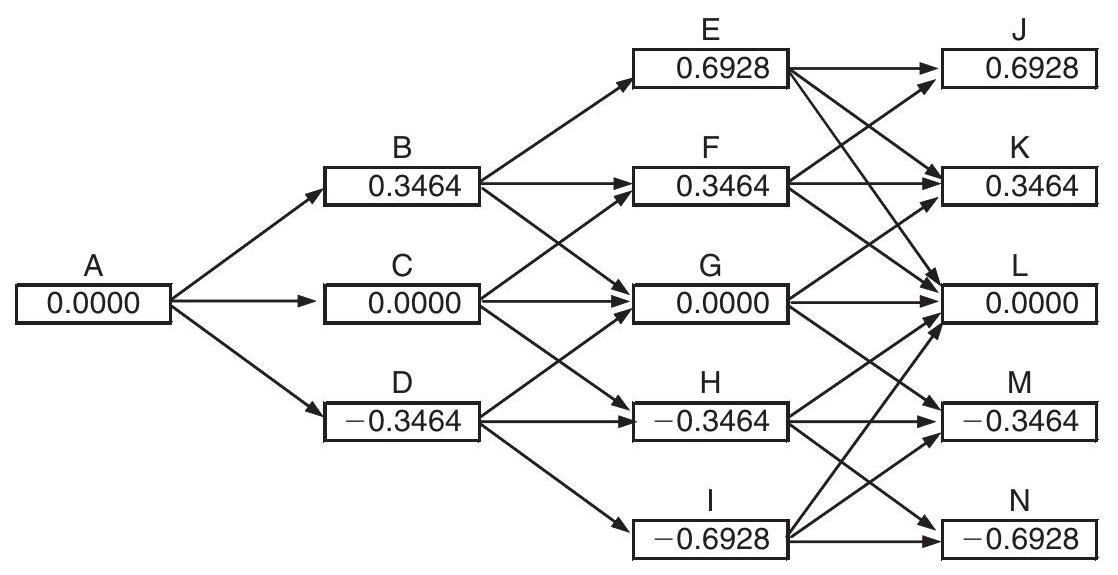
\includegraphics[width=0.31\linewidth]{da7d1f4c-f02d-4245-82cc-df26ce412cbf-791_575_1118_422_360.jpg}
        \hfill
        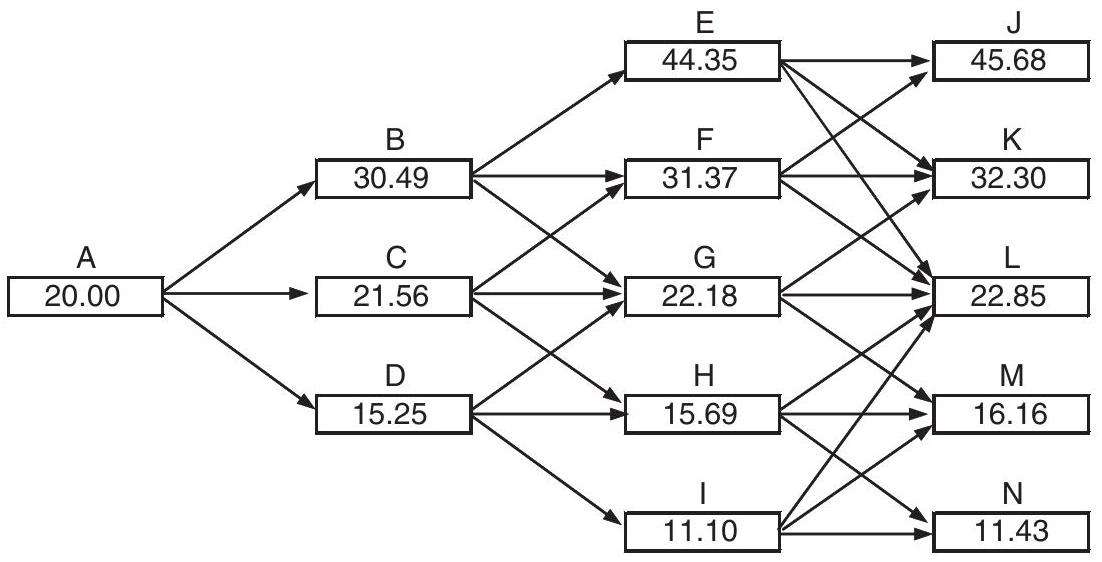
\includegraphics[width=0.31\linewidth]{da7d1f4c-f02d-4245-82cc-df26ce412cbf-792_562_1102_1460_455.jpg}
        \hfill
        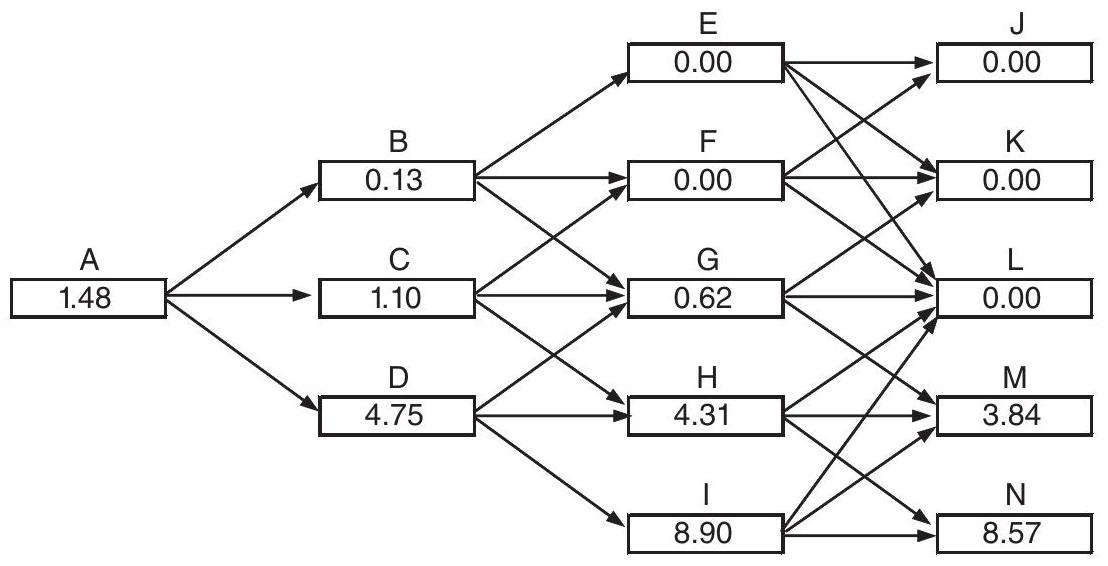
\includegraphics[width=0.31\linewidth]{da7d1f4c-f02d-4245-82cc-df26ce412cbf-793_566_1108_378_365.jpg}
    \end{center}
\end{frame}

\section{Stock Index Futures and Beta Hedging}

\begin{frame}{Intuition for Beta Hedging}
    \small
    \begin{block}{Core idea}
        A stock portfolio has \textbf{market exposure} and \textbf{stock-specific exposure}.
        Index futures mainly hedge the \textbf{market-wide} part.
    \end{block}

    \begin{itemize}
        \item Beta tells how strongly the portfolio tends to move with the index.
        \item A USD 40m portfolio with beta 1.25 behaves like about USD 50m of market exposure.
        \item If one futures contract gives USD 1m of index exposure, shorting 50 contracts offsets that market exposure.
        \item If the market falls, the portfolio loses but the short futures gain; if the market rises, the opposite happens.
        \item The manager can reduce market risk quickly without selling the underlying stocks.
    \end{itemize}

    \begin{alertblock}{What the hedge does not remove}
        Stock selection risk, sector tilts, changing beta, and futures basis risk can still remain.
    \end{alertblock}
\end{frame}

\begin{frame}{Stock-Index Futures and Beta Hedging}
    \small
    One index futures contract has value
    \[
        V_F=\text{futures price}\times \text{multiplier}.
    \]

    If a portfolio has beta $\beta$ relative to the index, the number of contracts to short is
    \[
        N^*=\beta\frac{V_A}{V_F}.
    \]

    \begin{exampleblock}{Full market hedge}
        Portfolio value: USD 40m, beta: 1.25, index futures: 4,000, multiplier: 250.
        Then
        \[
            V_F=4{,}000\times 250=1{,}000{,}000,
            \qquad
            N^*=1.25\frac{40{,}000{,}000}{1{,}000{,}000}=50.
        \]
        Short 50 contracts.
    \end{exampleblock}
\end{frame}

\begin{frame}{Changing Portfolio Beta}
    \small
    Futures can change exposure without selling the underlying stocks:
    \[
        N^*=(\beta-\beta^*)\frac{V_A}{V_F}.
    \]

    \begin{columns}[T]
        \begin{column}{0.48\textwidth}
            \begin{block}{Reduce beta}
                From 1.40 to 0.80 on a USD 25m portfolio with USD 250,000 per contract:
                \[
                    N^*=(1.40-0.80)\frac{25{,}000{,}000}{250{,}000}=60.
                \]
                Short 60 contracts.
            \end{block}
        \end{column}
        \begin{column}{0.48\textwidth}
            \begin{block}{Increase beta}
                From 0.70 to 1.10 on a USD 10m portfolio with USD 200,000 per contract:
                \[
                    N^*=(0.70-1.10)\frac{10{,}000{,}000}{200{,}000}=-20.
                \]
                Go long 20 contracts.
            \end{block}
        \end{column}
    \end{columns}

    \begin{alertblock}{Residual risk}
        Beta hedges remove broad market exposure only approximately.
        Stock selection, sector tilts, changing beta, dividends, liquidity, and basis risk remain.
    \end{alertblock}
\end{frame}

\section{Stack-and-Roll Hedging}

\begin{frame}{Stack-and-Roll Hedging}
    \begin{columns}[T]
        \begin{column}{0.52\textwidth}
            \begin{itemize}
                \item Use nearby liquid contracts when the exposure lasts longer than liquid futures maturities.
                \item Close the old contract and open a new one as maturity approaches.
                \item Each roll creates risk because the old and new contracts can move differently.
            \end{itemize}

            \begin{alertblock}{Risk-Management Lesson}
                Stack-and-roll can turn price risk into liquidity and funding risk because futures losses must be paid in cash before the physical exposure is realized.
            \end{alertblock}
        \end{column}
        \begin{column}{0.44\textwidth}
            \begin{center}
                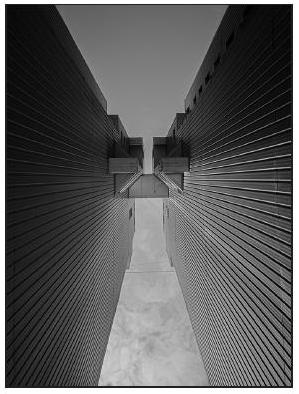
\includegraphics[width=\linewidth,height=0.62\textheight,keepaspectratio]{da7d1f4c-f02d-4245-82cc-df26ce412cbf-070_394_299_62_1457.jpg}
            \end{center}
        \end{column}
    \end{columns}
\end{frame}

\section{Wrap-Up}

\begin{frame}{What You Should Know After Lecture 2}
    \begin{itemize}
        \item Decide whether a hedge should be short or long.
        \item Compute effective hedge prices using the final basis.
        \item Explain why cross hedges need an estimated hedge ratio.
        \item Use futures to hedge or change stock-market beta.
        \item Derive forward prices from no-arbitrage with income, yield, storage, and convenience yield.
        \item Explain why futures prices are pricing objects, not automatically unbiased forecasts.
    \end{itemize}
\end{frame}

\begin{frame}{Practice Before Next Class}
    \begin{enumerate}
        \item Compute the effective price in a short hedge and in a long hedge.
        \item Estimate the minimum-variance hedge ratio from $\rho$, $\sigma_S$, and $\sigma_F$.
        \item Calculate the number of contracts for a stock-index beta hedge.
        \item Price a forward with no income, known income, and known yield.
        \item Explain when convenience yield can keep a commodity futures price below a simple cash-and-carry benchmark.
    \end{enumerate}
\end{frame}

\appendix

\begin{frame}[label=mvhr-appendix]{Appendix: Derivation of the Minimum-Variance Hedge Ratio}
    \footnotesize
    Start from the hedged change and choose \(h\) to minimize its variance:
    \[
        \begin{aligned}
            \Delta V &= \Delta S+h(-\Delta F)=\Delta S-h\Delta F, \\
            \Var(\Delta V)
            &= \Var(\Delta S-h\Delta F) \\
            &= \sigma_S^2+h^2\sigma_F^2-2h\Cov(\Delta S,\Delta F), \\
            \frac{d}{dh}\Var(\Delta V)
            &= 2h\sigma_F^2-2\Cov(\Delta S,\Delta F).
        \end{aligned}
    \]

    Set the derivative equal to zero and solve:
    \[
        \begin{aligned}
            0 &= 2h\sigma_F^2-2\Cov(\Delta S,\Delta F), \\
            h^*\sigma_F^2 &= \Cov(\Delta S,\Delta F), \\
            h^* &= \frac{\Cov(\Delta S,\Delta F)}{\Var(\Delta F)}.
        \end{aligned}
    \]

    Now use \(\Cov(\Delta S,\Delta F)=\rho\sigma_S\sigma_F\) and \(\Var(\Delta F)=\sigma_F^2\):
    \[
        h^*
        =
        \frac{\rho\sigma_S\sigma_F}{\sigma_F^2}
        =
        \rho\frac{\sigma_S}{\sigma_F}.
    \]

    \hyperlink{mvhr-main}{\beamerbutton{Back to main slide}}
\end{frame}

\end{document}
